% Setting common aspect ratios:
% - 169 for 16:9
% - 1610 for 16:10
% - 43 for 4:3
% - 32 for 3:2
% IMPORTANT: 
%	Aspect ratio may affect presentation quality! 
%	Make sure it fits your machine!
\documentclass[
	% 10pt, 
	aspectratio=1610,
]{beamer}

% Path to the watermark, cover in the title
% IMPORTANT: if cover figure is too small, magenta will appear!
\newcommand{\watermark}{figures/frontmatter/watermark.pdf}
\newcommand{\coverfigure}{figures/frontmatter/cover.pdf}

% Credits 
\newcommand{\watermarkcredit}{the authors}
\newcommand{\covercredit}{the authors}

% Figure is right justified, and will be horizontally/vertically offset by the amount below.
% Positive: figure goes to the right/up
% Negative: figure goest to the left/down
\newcommand{\coverXoffset}{0cm}
\newcommand{\coverYoffset}{0cm}

% Watermark is left justified, and will be horizontally/vertically offset by the amount below.
% Positive: watermark goes to the right/up
% Negative: watermark goest to the left/down
\newcommand{\watermarkXoffset}{0.8cm}
\newcommand{\watermarkYoffset}{-0.85cm}
\newcommand{\watermarkOpacity}{0.5} % Watermark opcity

\usetheme[
	sectionpages, 		% show section pages
	logo={figures/logo_UnB.pdf},
]{UniNA}

\usepackage[T1]{fontenc}
\usepackage[english]{babel} % if text is in portuguese, change "english" to "brazilian"

\usepackage[sfdefault]{carlito} % IMPORTANT: load carlito AFTER fontenc!

\usepackage{multicol}
\usepackage{multirow}
\usepackage{subcaption}

\usepackage{booktabs}
\usepackage{colortbl}
    \newcolumntype{L}[1]{>{\raggedright\let\newline\\\arraybackslash\hspace{0pt}}m{#1}}
    \newcolumntype{C}[1]{>{\centering\let\newline\\\arraybackslash\hspace{0pt}}m{#1}}
    \newcolumntype{R}[1]{>{\raggedleft\let\newline\\\arraybackslash\hspace{0pt}}m{#1}}

\usepackage{tikz}
    \usetikzlibrary{shapes,positioning,decorations.pathreplacing,arrows.meta,calc}
    \definecolor{verdeunb}{cmyk}{1,0,1,0.2}
    \definecolor{azulunb}{cmyk}{1,0.65,0,0.2}
    \definecolor{darkred}{HTML}{CA3A27}
    \definecolor{highlight}{HTML}{FFA300}
    \definecolor{steelblue}{HTML}{6EA4BF}

\usepackage{pgfplots}
    \pgfplotsset{compat=1.18}

% Erf special function rough approximation
\makeatletter
    \pgfmathdeclarefunction{erf}{1}{%
        \begingroup
            \pgfmathparse{#1 > 0 ? 1 : -1}%
            \edef\sign{\pgfmathresult}%
            \pgfmathparse{abs(#1)}%
            \edef\x{\pgfmathresult}%
            \pgfmathparse{1/(1+0.3275911*\x)}%
            \edef\t{\pgfmathresult}%
            \pgfmathparse{%
            1 - (((((1.061405429*\t -1.453152027)*\t) + 1.421413741)*\t 
            -0.284496736)*\t + 0.254829592)*\t*exp(-(\x*\x))}%
            \edef\y{\pgfmathresult}%
            \pgfmathparse{(\sign)*\y}%
            \pgfmath@smuggleone\pgfmathresult%
        \endgroup
    }
\makeatother
\providecommand{\e}[1]{\ensuremath{~\times~\text{10}^\text{#1}}}

\usepackage{bm}
\usepackage{bbm}

\usepackage{csquotes}
\usepackage{biblatex}
\addbibresource{references/main.bib}

\title[Gated DSI-ESMDA] %shown at the top of frames
{Gated Data-Space Inversion for\\ Reservoir Prediction} %shown in title frame
\subtitle[Reducing variance loss in posteriors]{Reducing variance loss in posteriors}  
\date[08/04/2026]{August 4th, 2026} %explicitly set date instead of \today

\author[Thiago]%shown at the top of frames
{%shown in title frame
	Thiago Tomás de Paula
}

\institute[%
	University of Brasília
]
{% is placed on the bottom of the title page
	Graduate students at
	University of Brasília, Brazil
}

\DeclareMathOperator*{\argmin}{\arg\!\min}
\DeclareMathOperator*{\argmax}{\arg\!\max}
\usepackage{empheq} % for boxing equations

% Flowchart colors
\colorlet{startstopcolor}{highlight!50}
\colorlet{processcolor}{steelblue!50}
\colorlet{iocolor}{verdeunb!30}
\colorlet{decisioncolor}{steelblue!25}

% Flowchart blocks
\tikzstyle{startstop} = [
    rectangle, 
    rounded corners, 
    minimum width=2cm, 
    minimum height=1cm,
    text centered, 
    draw=black, 
    fill=startstopcolor,
]
\tikzstyle{process} = [
    rectangle, 
    minimum width=2cm, 
    minimum height=1cm, 
    text centered, 
    draw=black, 
    fill=processcolor,
    trapezium stretches=true,
]
\tikzstyle{io} = [
    trapezium, 
    trapezium left angle=70, 
    trapezium right angle=110, 
    minimum width=2cm, 
    minimum height=1cm, 
    text centered, 
    draw=black, 
    fill=iocolor,
    trapezium stretches=true,
]
\tikzstyle{decision} = [
    diamond, 
    minimum width=1cm, 
    minimum height=1cm, 
    text centered, 
    draw=black, 
    fill=decisioncolor,
]

\usepackage{cleveref}

\begin{document}

\maketitle

% Optional agenda
% \begin{frame}{Agenda}{}
% 	\tableofcontents
% \end{frame}

\section{Introduction}

\begin{frame}{Introduction}{Context (graduate program)}
\end{frame}

\begin{frame}{Introduction}{Context (research)}
\end{frame}

\begin{frame}{Introduction}{The inverse problem}
\end{frame}

\begin{frame}{Introduction}{Literature review}
\end{frame}
\section{Theory Framework}

\begin{frame}{Theory Framework}{Important concepts and notation}
\end{frame}

\begin{frame}{Theory Framework}{Statistical framework}
\end{frame}

\begin{frame}{Theory Framework}{The base equation}
\end{frame}

\begin{frame}{Theory Framework}{Covariance localization}
\end{frame}

\begin{frame}{Theory Framework}{Proposal}
\end{frame}
\section{Methods}

\begin{frame}{Methods}
	\begin{itemize}
		\item Present the case studies - petrophysical properties of each reservoir
		\item Present the case studies - (normalized) field oil production total of each reservoir
		\item Present the workflow behind the experiments (including noise modeling)
		\item Present the evaluation metrics used (compare meanings)
		\item Present the time, localization and features parameters employed
	\end{itemize}
\end{frame}
\section{Results}

\begin{frame}{Results}{Egg case}
\end{frame}

\begin{frame}{Results}{Olympus case}
\end{frame}

\begin{frame}{Results}{Real field case}
\end{frame}

\begin{frame}{Results}{Discussion}
    \begin{block}{OC, MSE and mismatch increase}
        Increase in gating intensity tended to increase 
        observation coverage, mean squared error, and data mismatch,
        albeit with case-dependent sensitivities.
    \end{block}
    \vfill
    \def\arraystretch{2}
    \begin{tabular}{rp{0.9\linewidth}}
        $\triangleright$ & Gating reduces posterior variance loss, so increase in coverages, but also MSE and mismatch, are expected as gating intensifies.
    \\
        $\triangleright$ & Egg standard deviations are lesser than Olympus on two accounts:
        reservoir complexity, and ground-truth representativeness. Olympus' ground-truths were somewhat biased.
    \end{tabular}
    \vfill
\end{frame}

\begin{frame}{Results}{Discussion}
    \begin{block}{Mixed effects of localization}
        Localization yielded mixed results: for the Egg and real field cases,
        effects on coverage and MSE were minimal, especially for intense enough gatings,
        while the effect in the Olympus case was drastic.
        %
        % Cumulative distribution plots of the field oil production total suggest 
        % that ground-truths are unbiased in the Egg and real field cases,
        % but somewhat biased for the Olympus case.
    \end{block}
    \vfill
    \def\arraystretch{1.75}
    \begin{tabular}{rp{0.93\linewidth}}
        $\triangleright$ & 
        \textbf{Egg case}:
            narrow FOPT range and roughly uniform sampling of ground-truths leave no ground-truth unrepresented,
            reduced dimentionality help with covariance estimation.
    \\
        $\triangleright$ &
        \textbf{Olympus case}:
            much more complex while also having a much smaller ensemble
            and a lot more features, aggravating covariance estimation.
            Localization was conceived exactly for such situations, so it is not suprising it was effective here.
    \\
        $\triangleright$ &
        \textbf{Real field case}:
            peak complexity and dimentionality, but also ensemble size.
            Localization may have inadequately adjusted, and some features are not well-represented.
    \end{tabular}
\end{frame}

\begin{frame}{Results}{Discussion}
    \begin{figure}[h!]\centering
        \begin{subfigure}{.49\linewidth}\centering
            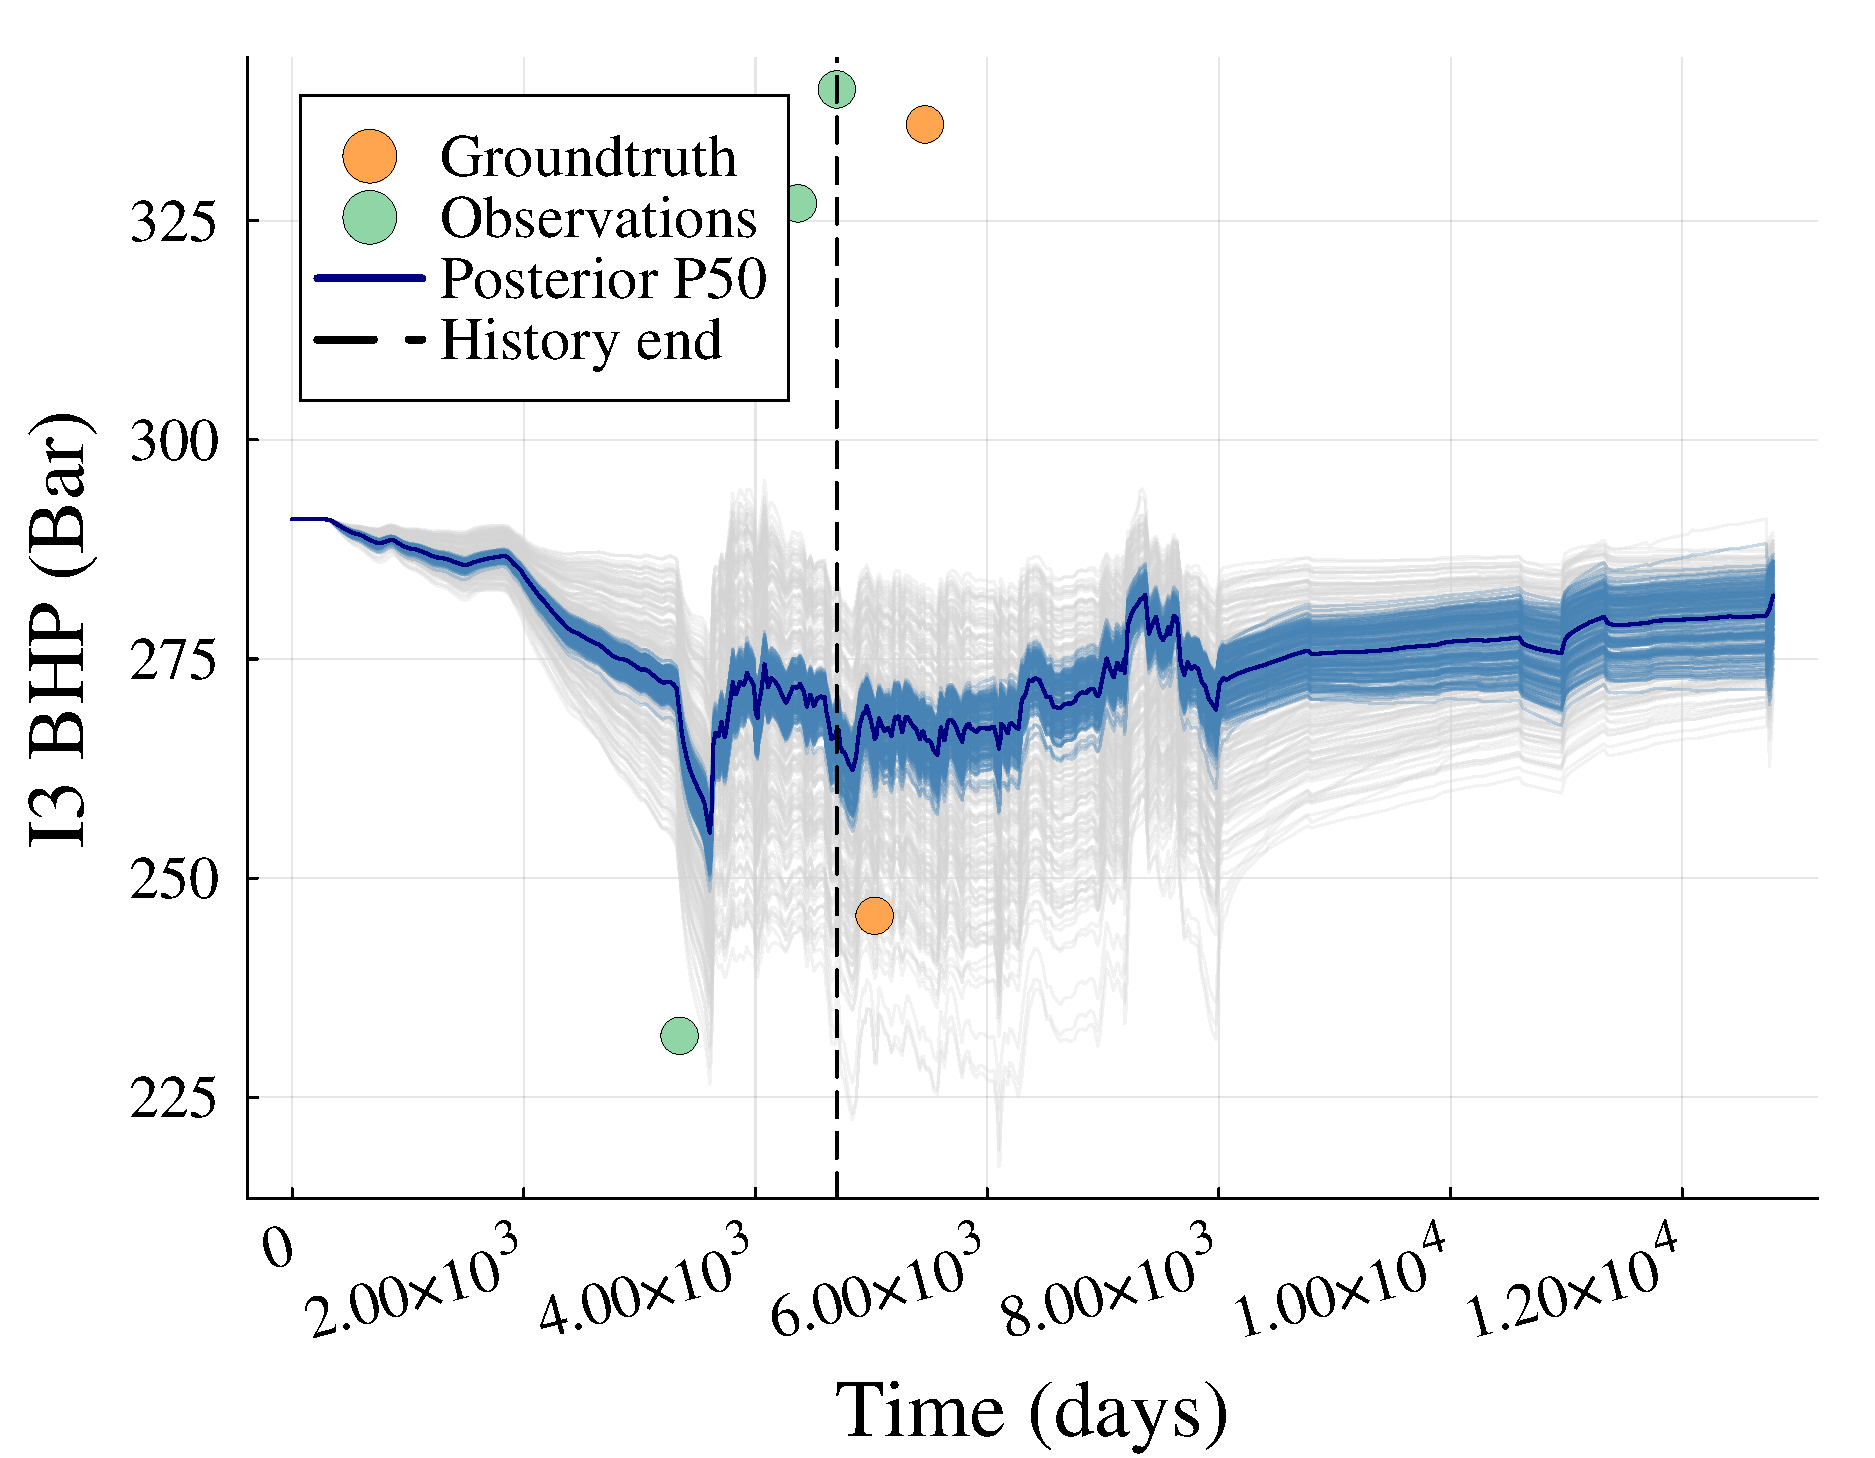
\includegraphics[width=0.775\linewidth]{figures/results/real_field/gt_0/noise_magnitude_0.01/n_iterations_1/localization_false/gating_true/gating_intensity_4.0/WELLS_I3_WBHP.pdf}
        \end{subfigure}  
        \begin{subfigure}{.49\linewidth}\centering
            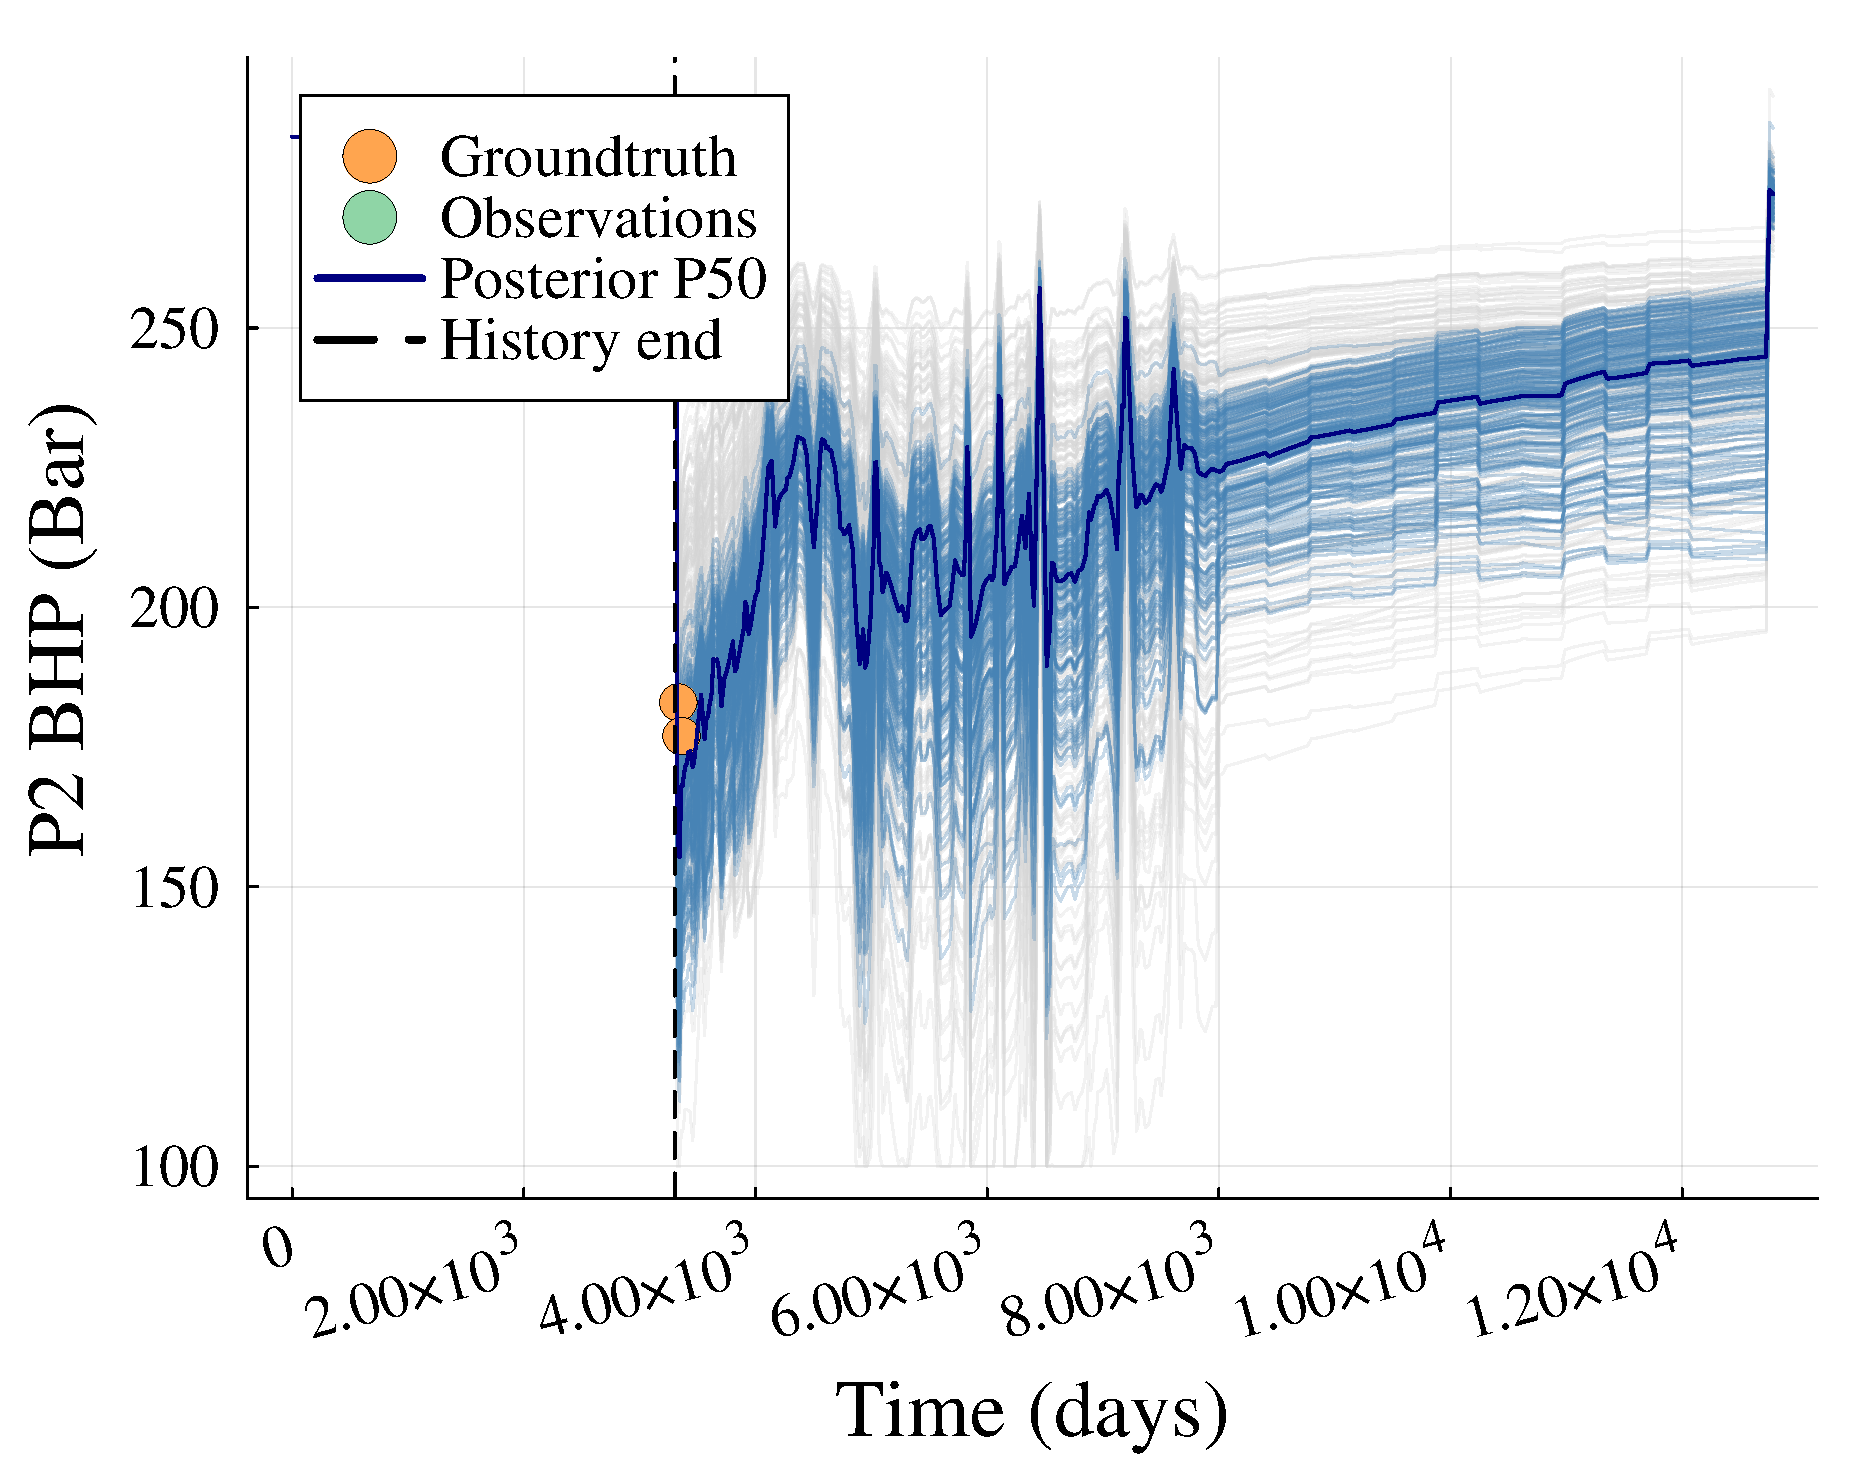
\includegraphics[width=0.775\linewidth]{figures/results/real_field/gt_0/noise_magnitude_0.01/n_iterations_1/localization_false/gating_true/gating_intensity_4.0/WELLS_P2_WBHP.pdf}
        \end{subfigure}
        \begin{subfigure}{.49\linewidth}\centering
            
\includegraphics[width=0.775\linewidth]{figures/results/real_field/gt_0/noise_magnitude_0.01/n_iterations_1/localization_false/gating_true/gating_intensity_4.0/WELLS_P11_WBHP.pdf}
        \end{subfigure}
        \begin{subfigure}{.49\linewidth}\centering
            
\includegraphics[width=0.775\linewidth]{figures/results/real_field/gt_0/noise_magnitude_0.01/n_iterations_1/localization_false/gating_true/gating_intensity_4.0/WELLS_P12_WBHP.pdf}
        \end{subfigure}
    \end{figure}
\end{frame}

\begin{frame}{Results}{Discussion}
    \begin{block}{Mild and small gating intensities versus standard DSI-ESMDA}
        Mild gating intensities (2 in the Egg and Olympus cases, 4 in the real field case) produced similar results 
        to the standard DSI-ESMDA for same localization configuration,
        while small gating (1 for the Egg case, 1 and 2 for the Olympus and real field cases)
        had worse coverages than the standard DSI-ESMDA.
    \end{block}
    \vfill
    \def\arraystretch{1.75}
    \begin{tabular}{rp{0.93\linewidth}}
        $\triangleright$ & 
        Gating intensity ``reverts'' the posterior to the prior.
        If the posterior given by the standard DSI-ESMDA is somewhere in that continuum,
        then it stands to reason that Gated DSI-ESMDA could approximate it simply by tuning the gating intensity.
    \\
        $\triangleright$ & 
        Since Gated DSI-ESMDA does away with observation data resampling,
        small gatings possibly underestimate uncertainty (i.e., likelihood covariance)
        at least when compared to standard DSI-ESMDA,
        producing posteriors that are not well-matched to data.
    \end{tabular}
\end{frame}
% \section{Conclusion}

\begin{frame}{Conclusion}
    \def\arraystretch{1.5}
    \begin{tabular}{l p{12cm}}
        $\triangleright$ &
            This work introduced Gated DSI-ESMDA, an extension of DSI-ESMDA 
            with a nonlinear innovation gating mechanism that increases posterior variance 
            the more intense the gating.
    \\
        $\triangleright$ &
            Observation coverages of the posterior increased with the gating intensity for all case studies,
            albeit under different sensitivities.
    \\
        $\triangleright$ &
        Small gatings tend to underestimate uncertatinty, while mild gatings produced similar results to standard DSI-ESMDA.
    \\
        $\triangleright$ &
            The gating mechanism in of itself can be easily adapted into model-space methods such as ES-MDA.
    \\
        $\triangleright$ &
            Gated DSI-ESMDA 
            remains susceptible to poor feature selection and localization tuning,
            as well as insuficient ground-truth representativeness, 
            high data dimentionality, and reduced ensemble size. 
            Future research should address these problems.
            % Feature selection and localization optimization are thought to be two of the main culprits behind
            % lukewarm results in the real field case, and future research could address these problems.
    \end{tabular}
\end{frame}

\begin{frame}[t,allowframebreaks]
   \frametitle{Bibliography}
   \printbibliography[heading=none]
\end{frame}

% Optional ending slide
\begin{frame}[noframenumbering]
	\usebeamertemplate{endpage}
\end{frame}

\end{document}
		